%%%%%%%%%%%%%%%%%%%%%%%%%%%%%%%%%%%%%%%%%%%%%%%%%%%%%%%%%%%%%%%%%%%%%%%%%%%%%%%%%%
\begin{frame}[fragile]\frametitle{}
\begin{center}
{\Large RLib}
\end{center}
\end{frame}


%%%%%%%%%%%%%%%%%%%%%%%%%%%%%%%%%%%%%%%%%%%%%%%%%%%%%%%%%%%%%%%%%%%%%%%%%%%%%%%%%%
\begin{frame}[fragile]\frametitle{Need}


\begin{center}
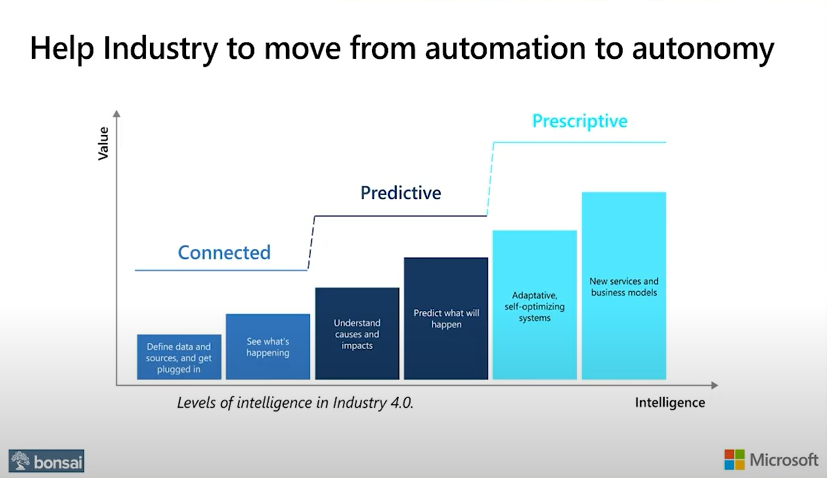
\includegraphics[width=\linewidth,keepaspectratio]{rl53}
\end{center}

{\tiny (Ref: Offline RL with RLlib - Edi Palencia)}

\end{frame}

%%%%%%%%%%%%%%%%%%%%%%%%%%%%%%%%%%%%%%%%%%%%%%%%%%%%%%%%%%%%%%%%%%%%%%%%%%%%%%%%%%
\begin{frame}[fragile]\frametitle{Solution}


\begin{center}
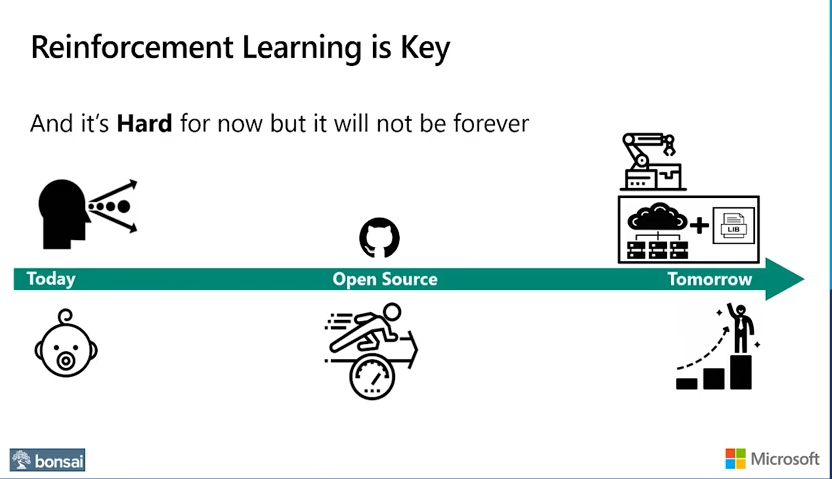
\includegraphics[width=0.8\linewidth,keepaspectratio]{rl54}
\end{center}

An Open Source Distributed Training Library for Reinforcement Learning == RLib.

{\tiny (Ref: Offline RL with RLlib - Edi Palencia)}

\end{frame}

%%%%%%%%%%%%%%%%%%%%%%%%%%%%%%%%%%%%%%%%%%%%%%%%%%%%%%%%%%%%%%%%%%%%%%%%%%%%%%%%%%
\begin{frame}[fragile]\frametitle{RLib}

\begin{center}
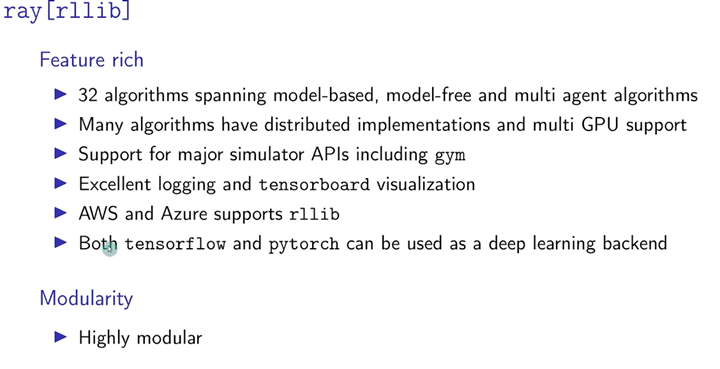
\includegraphics[width=\linewidth,keepaspectratio]{rl52}
\end{center}

{\tiny (Ref: Which Reinforcement Learning Framework is the Best?)}

\end{frame}

%%%%%%%%%%%%%%%%%%%%%%%%%%%%%%%%%%%%%%%%%%%%%%%%%%%%%%%%%%%%%%%%%%%%%%%%%%%%%%%%%%
\begin{frame}[fragile]\frametitle{RLib and Ray}


\begin{center}
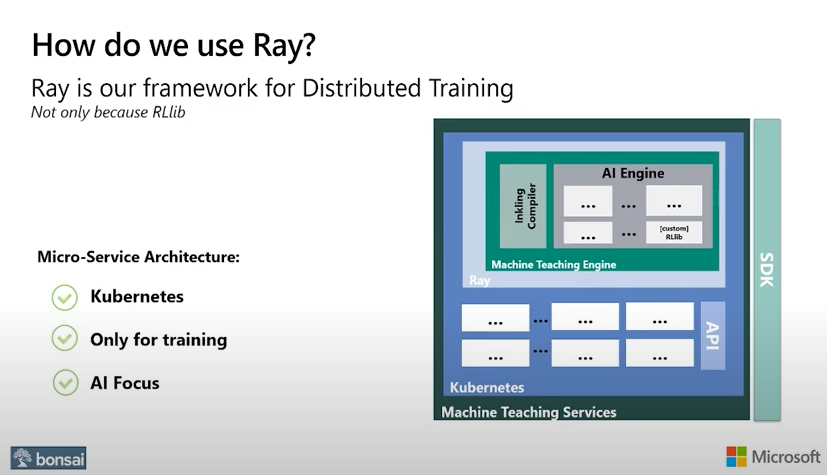
\includegraphics[width=0.8\linewidth,keepaspectratio]{rl55}
\end{center}

RLib is part of overall Ray framework.

{\tiny (Ref: Offline RL with RLlib - Edi Palencia)}

\end{frame}

%%%%%%%%%%%%%%%%%%%%%%%%%%%%%%%%%%%%%%%%%%%%%%%%%%%%%%%%%%%%%%%%%%%%%%%%%%%%%%%%%%
\begin{frame}[fragile]\frametitle{Installation}
\begin{itemize}
\item Needs Pytorch or Tensorflow at the back-end. Install either in the rl environment.
\item \lstinline|pip install ray[rllib]|
\item  Check by:

\begin{lstlisting}
import ray

ray.init()

RayContext(dashboard_url='', python_version='3.9.12', ray_version='1.13.0', ...})
\end{lstlisting}
\end{itemize}
\end{frame}

%%%%%%%%%%%%%%%%%%%%%%%%%%%%%%%%%%%%%%%%%%%%%%%%%%%%%%%%%%%%%%%%%%%%%%%%%%%%%%%%%%
\begin{frame}[fragile]\frametitle{Steps: Example: Cart Pole}
Need 
\begin{itemize}
\item A RL environment (e.g. CartPole-v1), This is Open AI Gym Env, but its integration with Ray lets us use the name directly.
\item A RL algorithm to learn in that environment (e.g. Proximal Policy Optimization (PPO))
\item Configuration (algorithm config, experiment config, environment config etc.)
\item An experiment runner (called tune)
\end{itemize}

\begin{lstlisting}
from ray import tune

tune.run("PPO",
         config={"env": "CartPole-v1",
                 # other configurations go here, if none provided, then default configurations will be used
                 }
         )
\end{lstlisting}

Experiment starts \ldots
\end{frame}

%%%%%%%%%%%%%%%%%%%%%%%%%%%%%%%%%%%%%%%%%%%%%%%%%%%%%%%%%%%%%%%%%%%%%%%%%%%%%%%%%%
\begin{frame}[fragile]\frametitle{Configuration}
Need 
\begin{itemize}
\item Common config
\item Algorithm specific config (overrides common config)
\item User defined config
	\begin{itemize}
	\item Alternate Training and Evaluation phases
	\item In Training, policy is optimized
	\item In Evaluation the policy is evaluated for goal
	\item Set `evaluation\_*' to adjust the length, as below
	\end{itemize}
\end{itemize}


\begin{lstlisting}
tune.run("PPO",
         config={"env": "CartPole-v1",
                 "evaluation_interval": 2,    # num of training iter between evaluations
                 "evaluation_num_episodes": 20,
                 "num_gpus": 0
                 }
         )
\end{lstlisting}

Experiment starts \ldots Look at evaluation text to see how the algorithm faired.

\end{frame}

%%%%%%%%%%%%%%%%%%%%%%%%%%%%%%%%%%%%%%%%%%%%%%%%%%%%%%%%%%%%%%%%%%%%%%%%%%%%%%%%%%
\begin{frame}[fragile]\frametitle{Visualize Results}
Need 
\begin{itemize}
\item Running logs are kept in a dir, which Tensorboard can visualize
\item An experiment creates the following files and folders in the results directory
\end{itemize}

\begin{lstlisting}
<results dir>
- PPO    # algorithm name
    |---- basic-variant-state-2021-06-11_16-01-54.json
    |---- experiment_state-2021-06-11_16-01-54.json
    |---- PPO_CartPole-v1_9424e_00000_0_2021-06-11_16-01-54    # training and evaluation data
        |---- events.out.tfevents.1623420114.devbox-x299
        |---- params.json
        |---- params.pkl
        |---- progress.csv
        |---- result.json
				
>tensorboard --logdir myfolder						
\end{lstlisting}


\end{frame}

%%%%%%%%%%%%%%%%%%%%%%%%%%%%%%%%%%%%%%%%%%%%%%%%%%%%%%%%%%%%%%%%%%%%%%%%%%%%%%%%%%
\begin{frame}[fragile]\frametitle{Visualize Results}

Go to the returned url in browser and see Training and Evaluation progress


\begin{center}
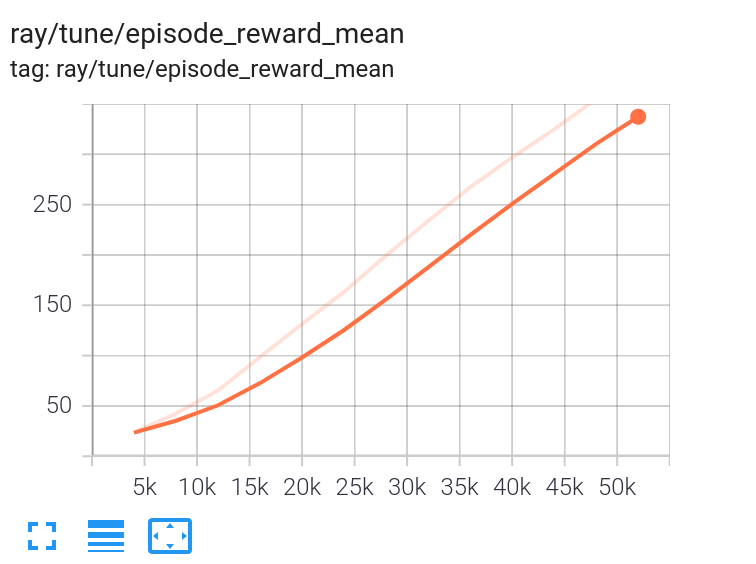
\includegraphics[width=0.6\linewidth,keepaspectratio]{rl64}

{\tiny (Ref: Fast RL - Dibya Chakraborty)}
\end{center}

Steps on X axis and chosen parameter on Y. You can pass data for multiple experiments with different algos, parameters, etc.

\end{frame}

%%%%%%%%%%%%%%%%%%%%%%%%%%%%%%%%%%%%%%%%%%%%%%%%%%%%%%%%%%%%%%%%%%%%%%%%%%%%%%%%%%
\begin{frame}[fragile]\frametitle{Save}

\begin{itemize}
\item Save the Agent to be used later
\item For that, crate Checkpoints during the experiment run
\item Set \lstinline|checkpoint_freq=2| in the config
\item Checkpoint save all information to restore the current policy.
\item Once goal is reached, manually stop.
\end{itemize}

\begin{center}

\includegraphics[width=0.4\linewidth,keepaspectratio]{rl65}
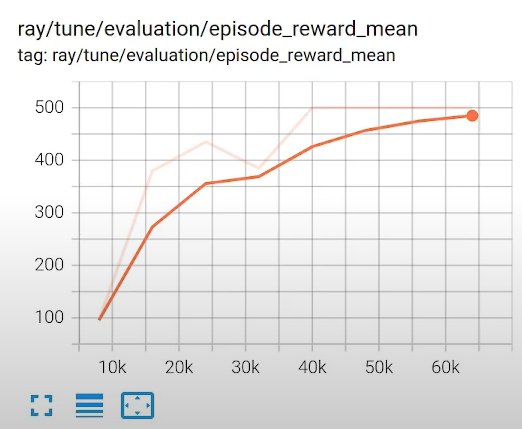
\includegraphics[width=0.4\linewidth,keepaspectratio]{rl66}

{\tiny (Ref: Fast RL - Dibya Chakraborty)}
\end{center}
\end{frame}

%%%%%%%%%%%%%%%%%%%%%%%%%%%%%%%%%%%%%%%%%%%%%%%%%%%%%%%%%%%%%%%%%%%%%%%%%%%%%%%%%%
\begin{frame}[fragile]\frametitle{Restore Agent}

\begin{itemize}
\item Import the trainer class.
\item Create an empty agent by initializing the trainer class. Use the same configuration as the experiment.
\item Restore the agent from the checkpoint.
\end{itemize}

% \begin{center}
% 
\includegraphics[width=0.4\linewidth,keepaspectratio]{rl67}

% {\tiny (Ref: Fast RL - Dibya Chakraborty)}
% \end{center}

\begin{lstlisting}

from ray.rllib.agents.ppo.ppo import PPOTrainer

agent = PPOTrainer(config={"env": "CartPole-v1",
                           "evaluation_interval": 2,
                           "evaluation_num_episodes": 20
                           }
                   )
agent.restore("../../checkpoint-16")
\end{lstlisting}

\end{frame}

%%%%%%%%%%%%%%%%%%%%%%%%%%%%%%%%%%%%%%%%%%%%%%%%%%%%%%%%%%%%%%%%%%%%%%%%%%%%%%%%%%
\begin{frame}[fragile]\frametitle{Use Agent}

Compute the action (according to the trained policy) using the \lstinline|agent.compute_action()| method

\begin{lstlisting}
import gym

env = gym.make("CartPole-v1")
obs = env.reset()
while True:
    action = agent.compute_action(obs)
    obs, reward, done, _ = env.step(action)
    env.render()
    if done:
        break
env.close()
\end{lstlisting}

\end{frame}

%%%%%%%%%%%%%%%%%%%%%%%%%%%%%%%%%%%%%%%%%%%%%%%%%%%%%%%%%%%%%%%%%%%%%%%%%%%%%%%%%%
\begin{frame}[fragile]\frametitle{Record Video}

Wrap the env in the \lstinline|gym.wrappers.RecordVideo| class and Supply the directory to write the video.

\begin{lstlisting}
from gym.wrappers import RecordVideo

env = RecordVideo(gym.make("CartPole-v1"), "ppo_video")
obs = env.reset()
while True:
    action = agent.compute_action(obs)
    obs, reward, done, _ = env.step(action)
    if done:
        break
env.close()
\end{lstlisting}

\end{frame}